\documentclass[final]{beamer}
% beamer 3.10: do NOT use option hyperref={pdfpagelabels=false} !
% \documentclass[final,hyperref={pdfpagelabels=false}]{beamer} 
% beamer 3.07: get rid of beamer warnings

\mode<presentation> {  
%% check http://www-i6.informatik.rwth-aachen.de/~dreuw/latexbeamerposter.php for examples
  \usetheme{Durham} %% This points to the theme cooked up by the final year tutor
}


\setbeamertemplate{caption}[numbered]
\usepackage[english]{babel} 
\usepackage[latin1]{inputenc}
\usepackage{amsmath,amsthm, amssymb, latexsym}
\usepackage{caption}
\usepackage{tabu}
\usepackage{graphicx}
\usepackage{harvard}

  \usefonttheme[onlymath]{serif}
  \boldmath
  \usepackage[orientation=portrait,size=a3,scale=1.4,debug]{beamerposter}                       

  % e.g. for DIN-A0 poster
  % \usepackage[orientation=portrait,size=a1,scale=1.4,grid,debug]{beamerposter}
  % e.g. for DIN-A1 poster, with optional grid and debug output
  % \usepackage[size=custom,width=200,height=120,scale=2,debug]{beamerposter} % e.g. for custom size poster
  % \usepackage[orientation=portrait,size=a0,scale=1.0,printer=rwth-glossy-uv.df]{beamerposter}
  % e.g. for DIN-A0 poster with rwth-glossy-uv printer check ...
  %

  \title[Final Year Project Poster]{Time Frame Trading Algorithms}
  \author[A L Gillies]{A. L. Gillies}
  \institute[Durham]{School Computing Sciences, Durham University}
  \date{16th April 2012}

  \begin{document}
  \begin{frame}{} 
  
  	\begin{block}{\large \centering When would you buy and sell?}
  	
  	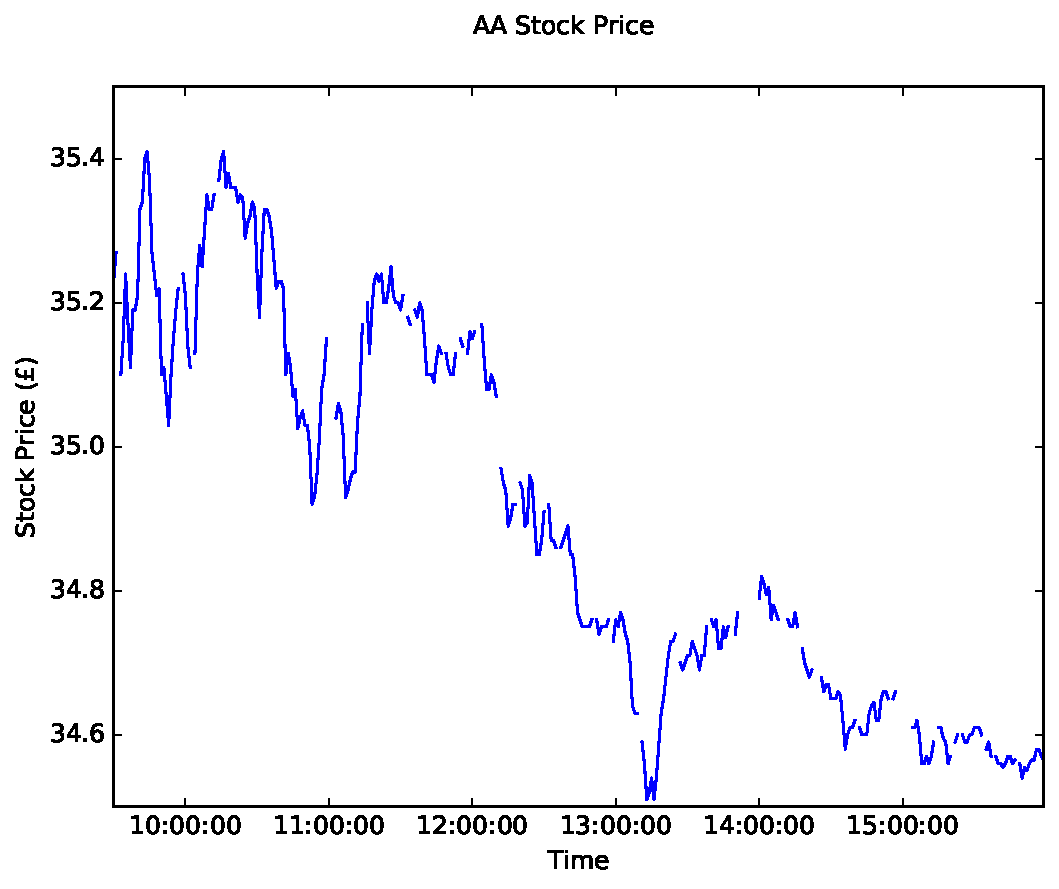
\includegraphics[width=0.23\columnwidth]{../AA.pdf} \hspace{10pt}
  	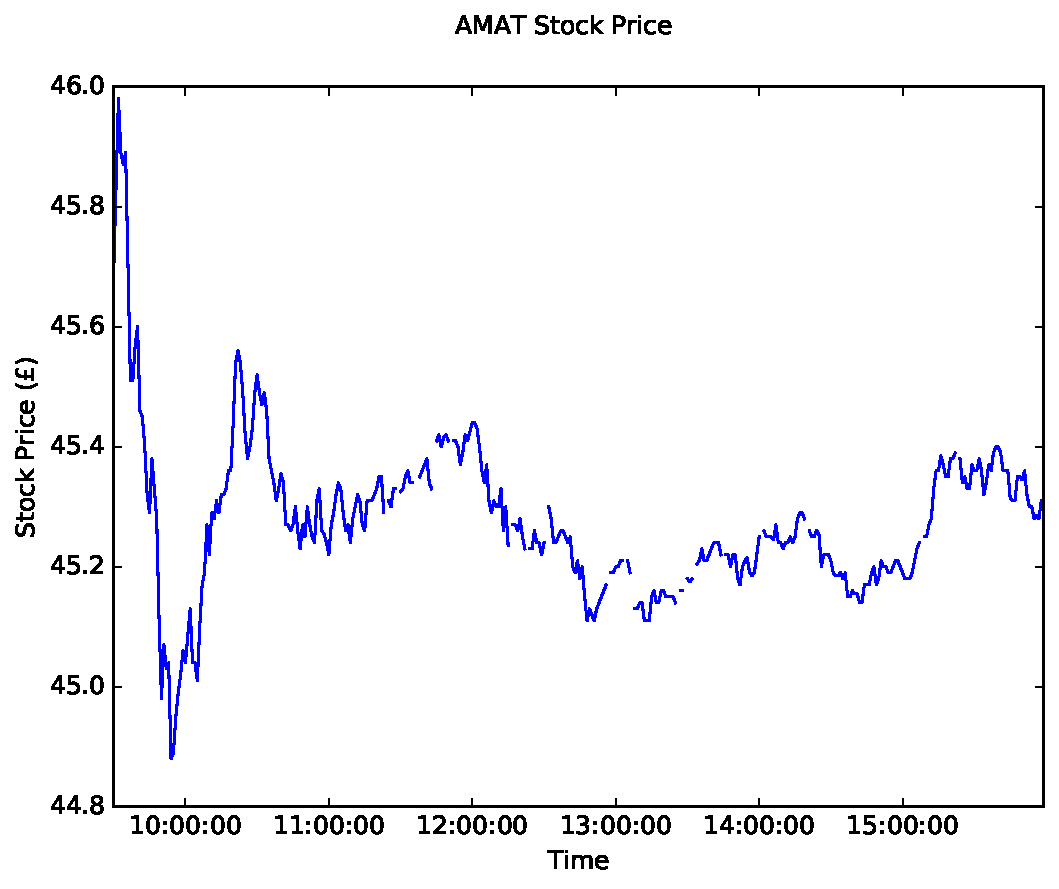
\includegraphics[width=0.23\columnwidth]{../AMAT.pdf} \hspace{10pt}
  	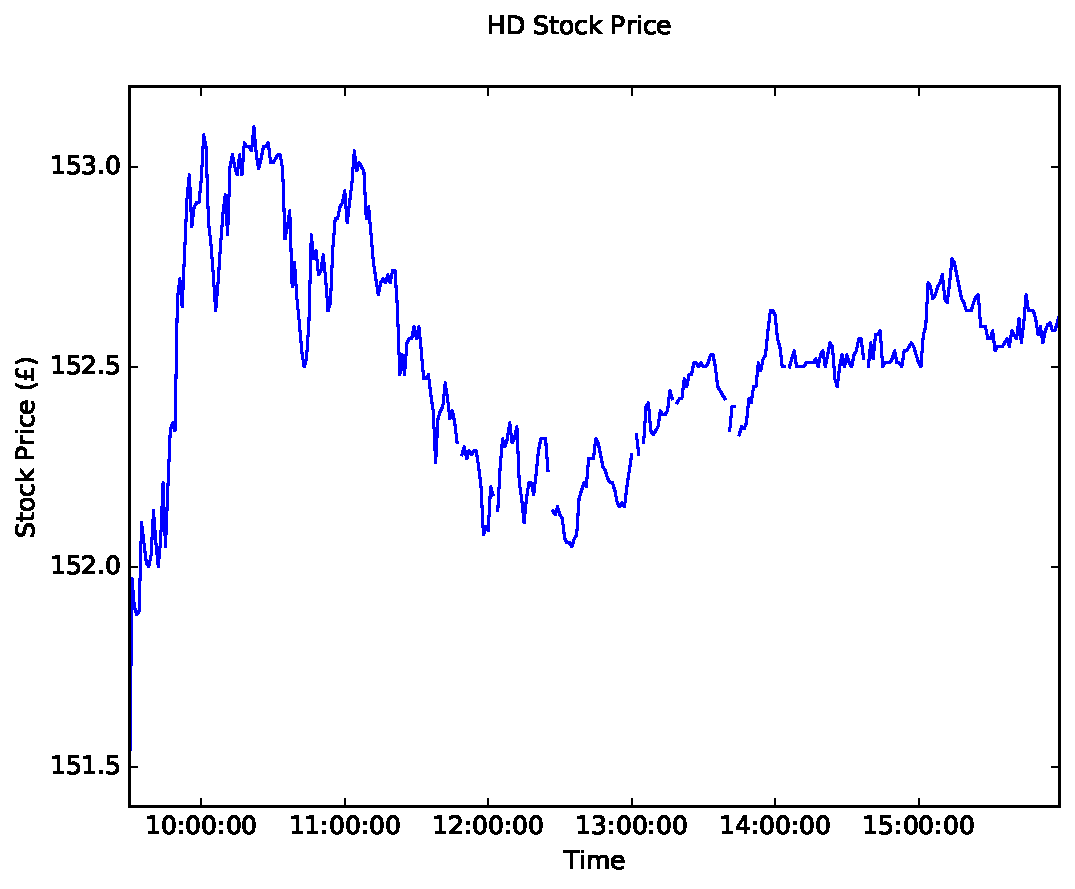
\includegraphics[width=0.23\columnwidth]{../HD.pdf} \hspace{10pt}
  	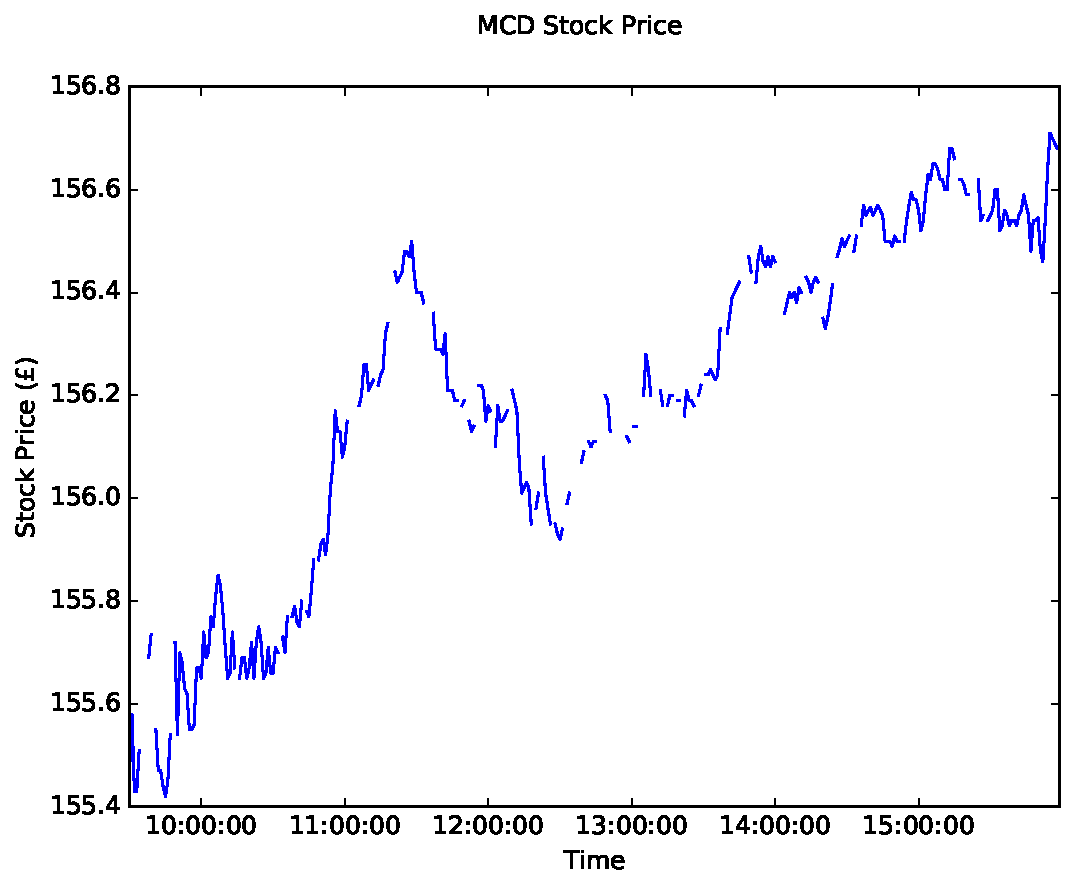
\includegraphics[width=0.23\columnwidth]{../MCD.pdf} \hspace{10pt}
  	
  	\end{block}
  	

    \begin{columns}[t]
    
 %%%%%%%%%%%%%%%%%%%%%%%%%%%%%%%%%%%%%%%%%%%%%
    
      \begin{column}{.48\linewidth}
      
%%%%%%%%%%%%%%%%%%%%%%%%
      
        \begin{block}{Introduction}
          Algorithmic trading is characterised by an entirely hands off approach to stock trading. Using this technique, can the average interest rate of high street banks, standing at 1.85\% (Murray 2018), be beaten? Two possibilities will be tested, statistical methodology and a machine learning based approach. 
        \end{block}
        
%%%%%%%%%%%%%%%%%%%%%%%%
        
        \begin{block}{Simulation}
        \begin{figure}
        \centering
		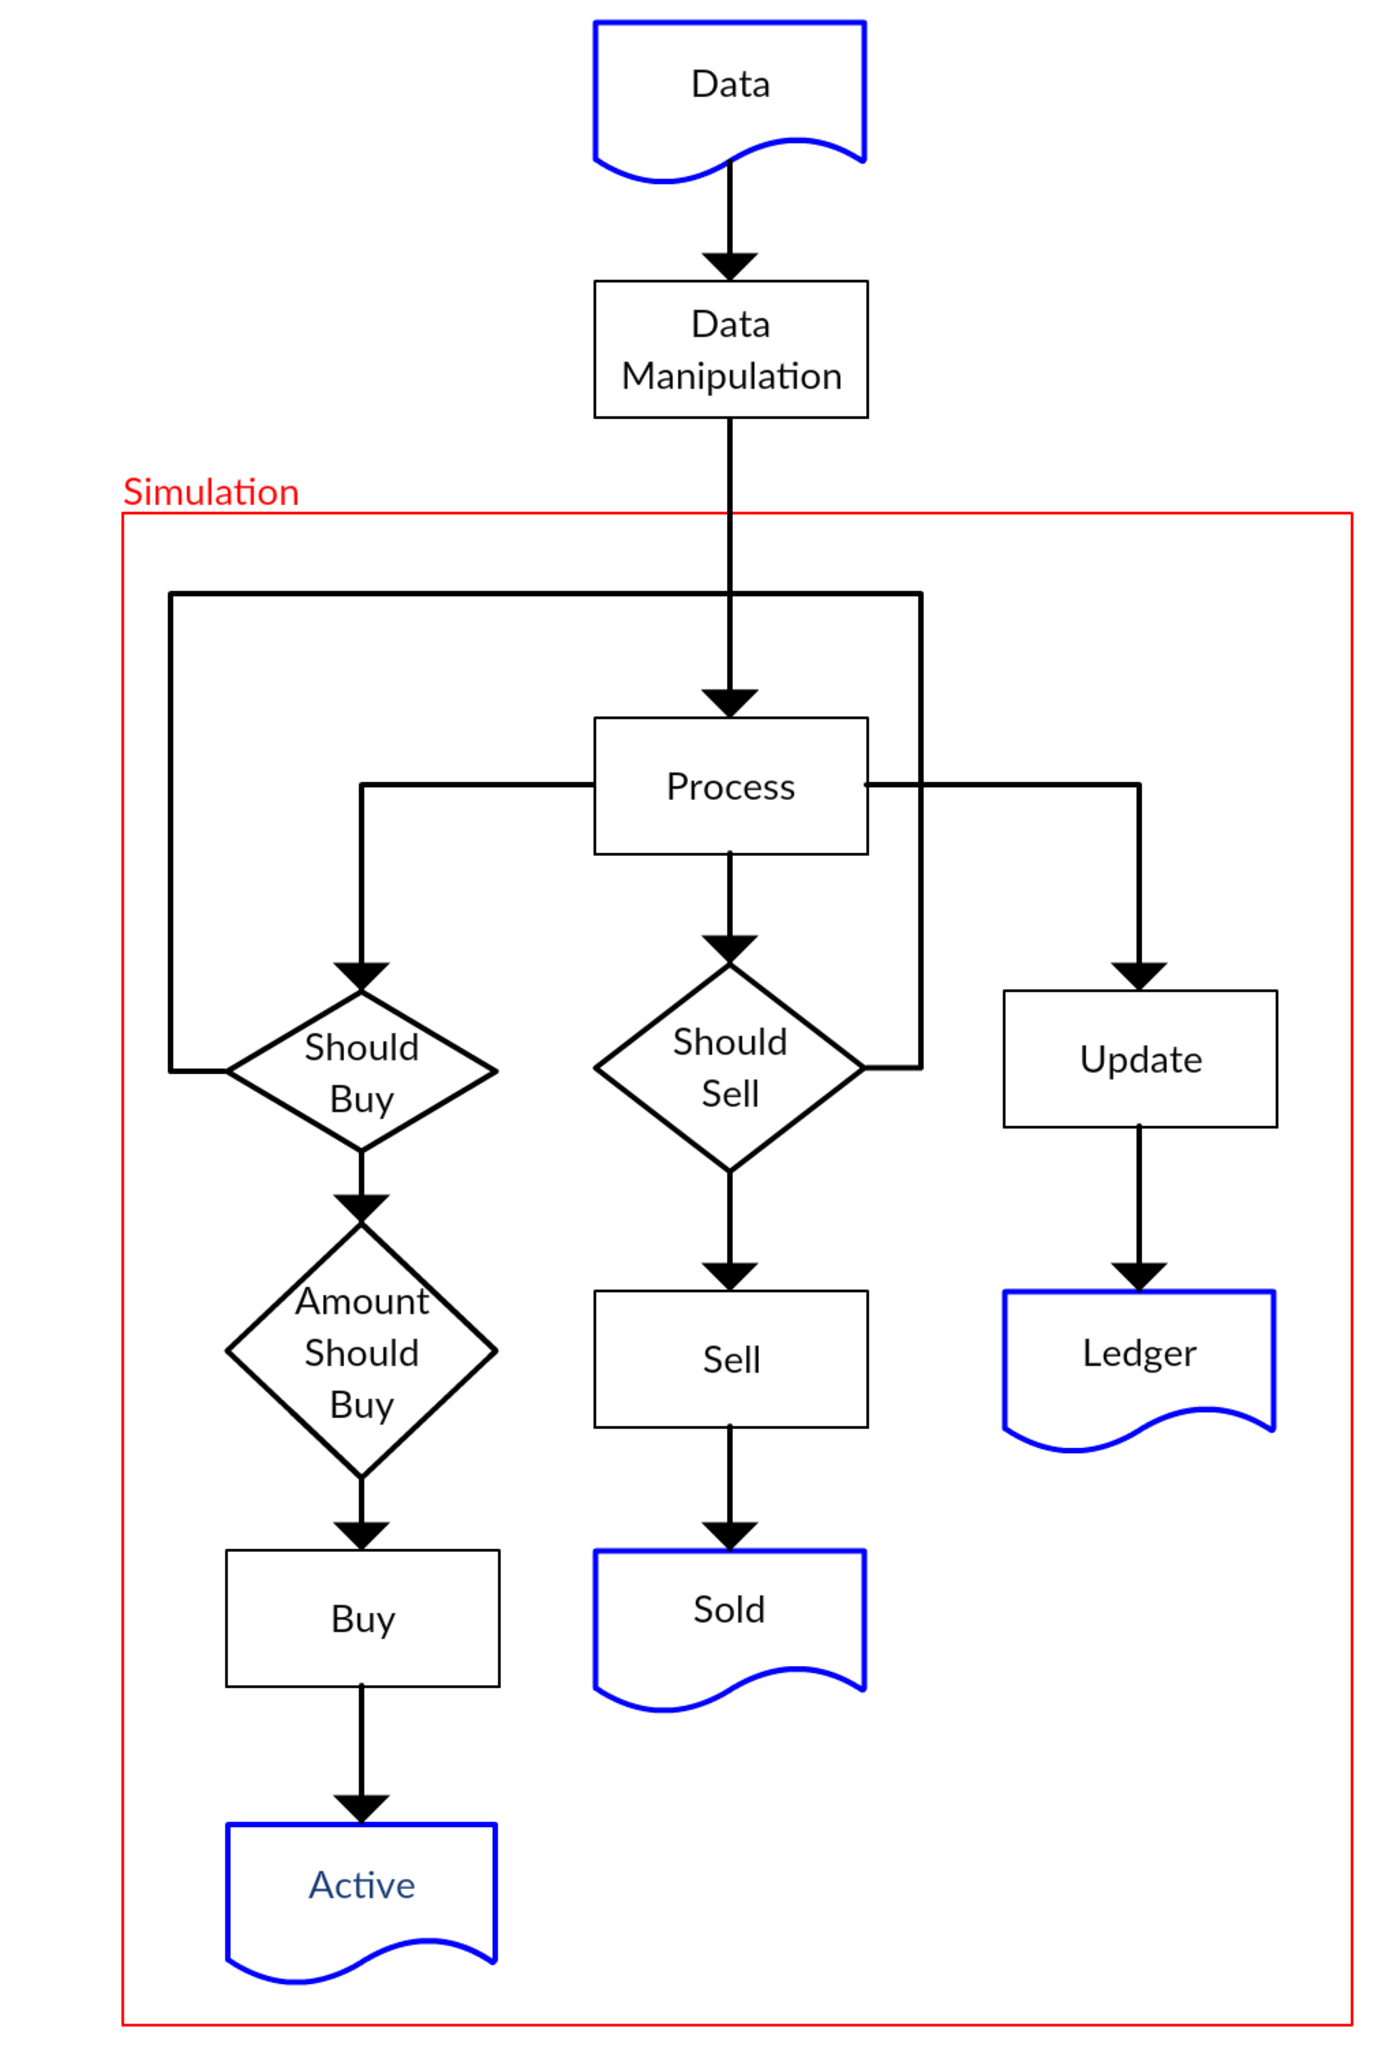
\includegraphics[width=0.4\columnwidth]{simFlow.pdf}
		\label{fig: SimFlow}
		\caption{A flow diagram showing the underlying logic of the simulation.}
		\end{figure}
        \end{block}
        
%%%%%%%%%%%%%%%%%%%%%%%%
        
        \begin{block}{Machine Learning Approach}
         
         \begin{columns}[t]
         
         \begin{column}{0.48\linewidth}
         
         \begin{figure}
         \centering
		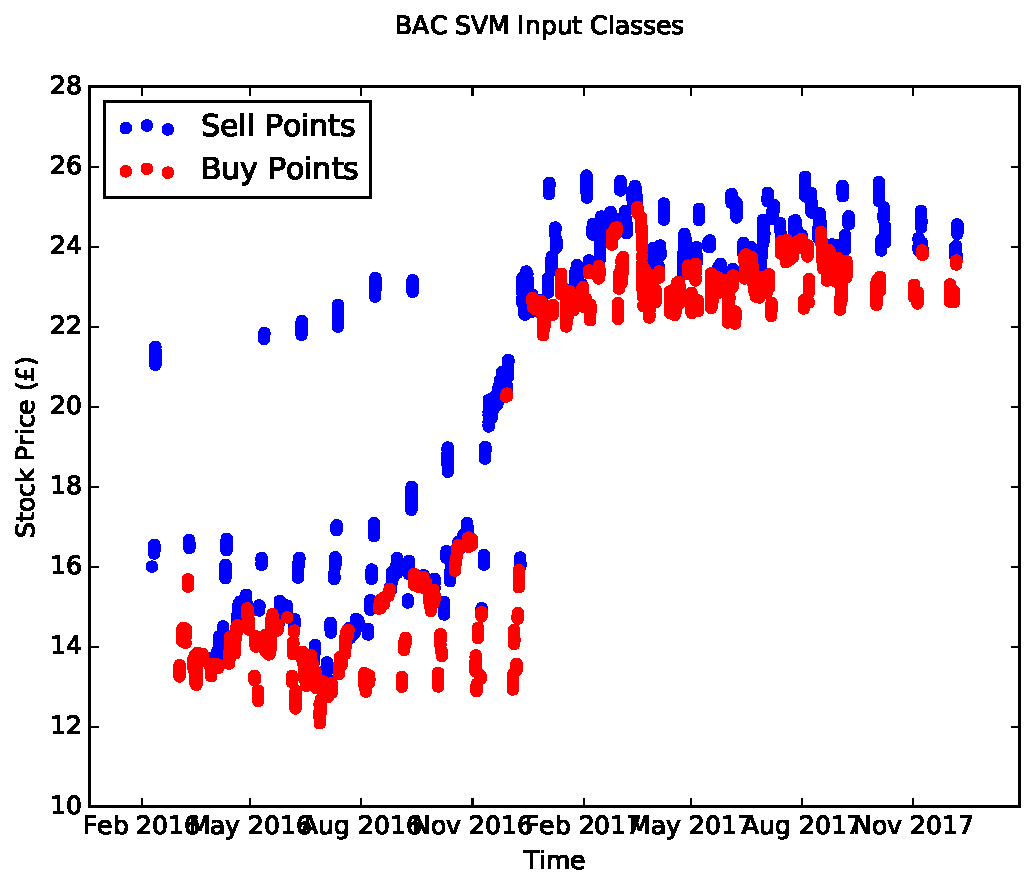
\includegraphics[width=0.95\columnwidth]{SVMBuyPoints.pdf}
		\caption{A flow diagram showing the underlying logic of the simulation.}
		\label{fig: SVMDataInput}
		\end{figure}
         
         \end{column}
         
         \begin{column}{0.42\linewidth}
         
         The input data for a support vector machine or SVM will allow for this shallow machine learning approach to maximise the support vectors or distance between two classifications of data. An example of this data separation is shown in Figure \ref{fig: SVMDataInput}. 
         
         \end{column}   
         
         \end{columns}
		
		\begin{figure}
         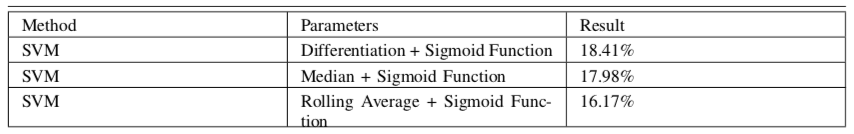
\includegraphics[width=0.8\columnwidth]{table3}
         \caption{The results of different SVM configurations.}
         \label{table: SVM Results}
         \end{figure}
		
		\end{block}

%%%%%%%%%%%%%%%%%%%%%%%%

		\begin{block}{References}
		
		\tiny
		Bollinger, J. (1992), `Using Bollinger Bands', Stocks \& Commodities 10(2), 47-51. \\
		Murray, A. (2018), `Fixed-rate accounts reach two-year highs: here are the best'. \\
		URL: https://www.telegraph.co.uk/investing/bonds/our-pick-of-the-best-
fixed-rate-savings-bonds
		
		\end{block}
        
%%%%%%%%%%%%%%%%%%%%%%%%

      \end{column}

%%%%%%%%%%%%%%%%%%%%%%%%%%%%%%%%%%%%%%%%%%%%%

      \begin{column}{.48\linewidth}
        
%%%%%%%%%%%%%%%%%%%%%%%%
        
         \begin{block}{Statistical Approach}
         
         \begin{columns}[t]
         
         \begin{column}{0.48\linewidth}
         
         \begin{figure}[h!]
         \centering
         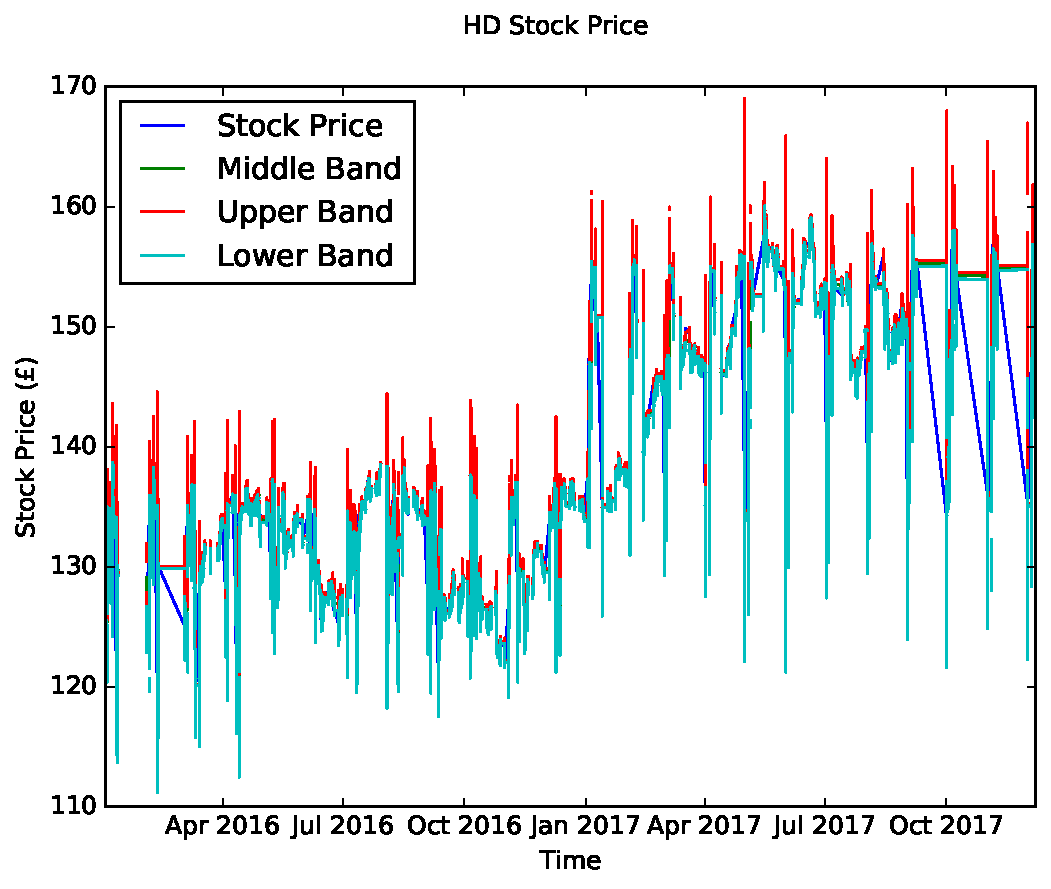
\includegraphics[width=0.95\columnwidth]{../HDYearBollinger.pdf}
         \caption{Showing the change in Bollinger Bands over a year.}
         \label{fig: HDYearBollinger}
         \end{figure}
         
         \begin{figure}[h!]
         \centering
         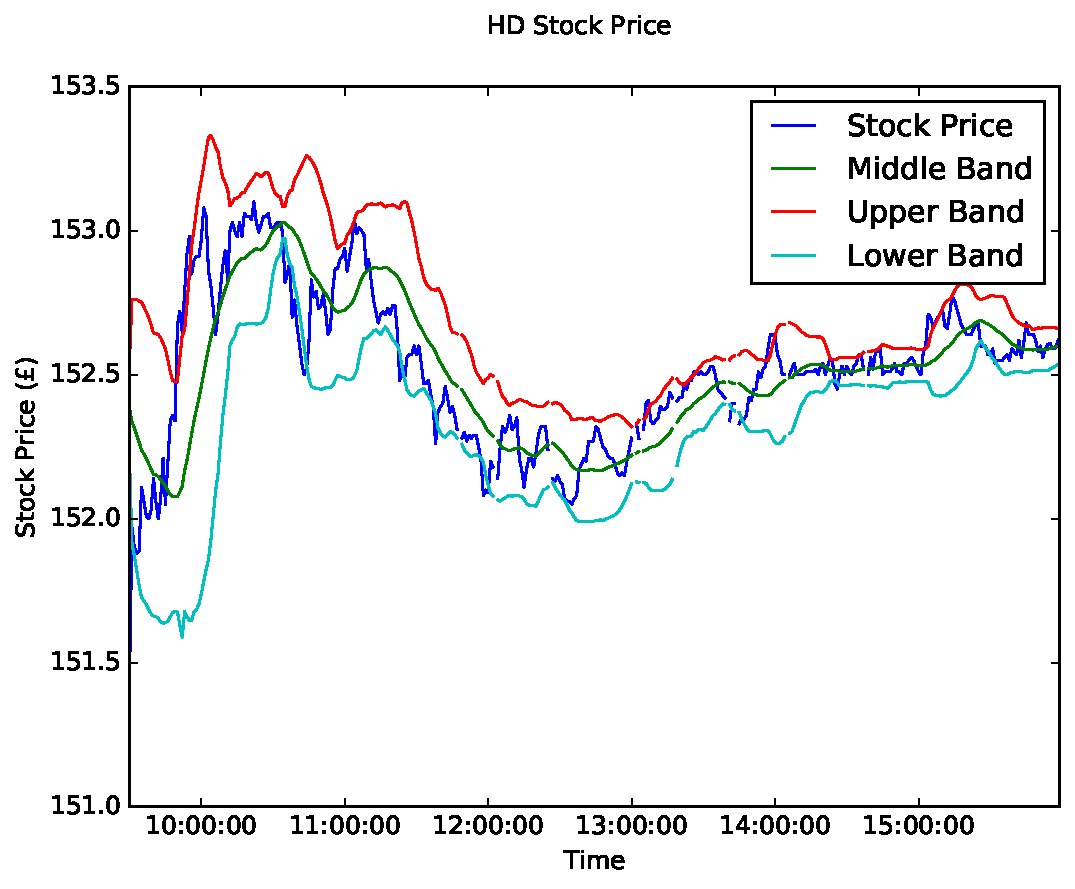
\includegraphics[width=0.95\columnwidth]{../HDDayBollinger.pdf}
         \caption{Showing the change in Bollinger Bands over a day.}
         \label{fig: HDDayBollinger}
         \end{figure}
         
         \end{column}
         
         \begin{column}{0.42\linewidth}
         
         An example of statistical methodology; the Bollinger Band, (Bollinger 1992). This statistical method is based around the work performed by John Bollinger on the volatility measures of stock market data. This method falls into the category of technical overlay, this is a method with an output value range that is dependant on the range of the input value. This, along with 9 other technical overlays and 27 technical indicators made up the statistical methods that were implemented and tested. A technical indicator is uniquely different to a technical overlay in that the input value range has no bearing on the range of the output values. The change in the range of the output is shown Figures \ref{fig: HDYearBollinger} and \ref{fig: HDDayBollinger}
         
         \end{column}
         
         \end{columns}

        \end{block}
        
%%%%%%%%%%%%%%%%%%%%%%%%
        
         \begin{block}{Results - Statistical Approach}
         
		 \begin{figure}
         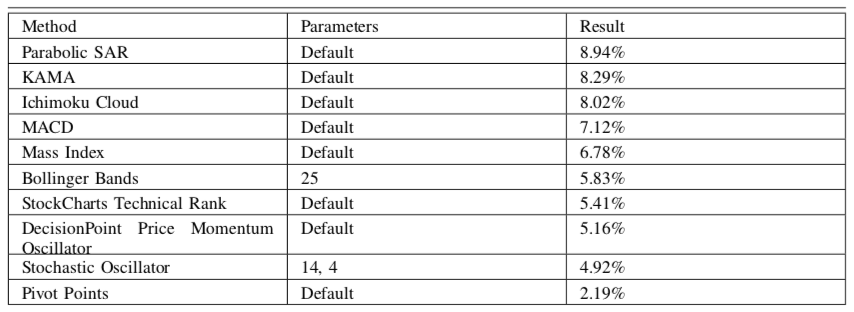
\includegraphics[width=0.8\columnwidth]{table1}
         \caption{The results of individual statistical methods.}
         \label{table: Individual Results}
         \end{figure}
         
         \begin{figure}
         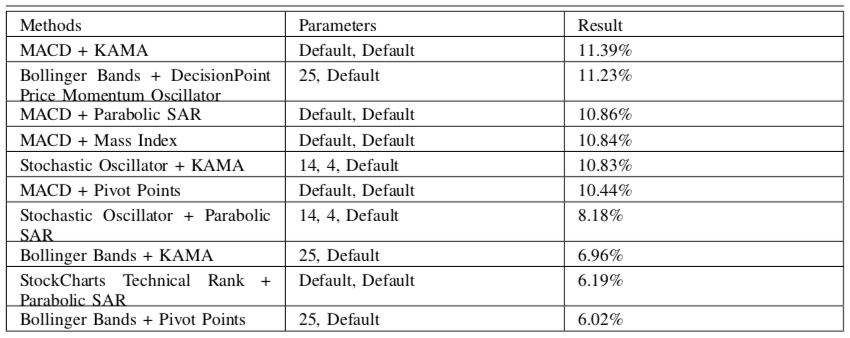
\includegraphics[width=0.8\columnwidth]{table2}
         \caption{The results of a conjunction of 2 or more statistical methods.}
         \label{table: Conjunction Results}
         \end{figure}

        \end{block}
        
%%%%%%%%%%%%%%%%%%%%%%%%

      \end{column}
      
%%%%%%%%%%%%%%%%%%%%%%%%%%%%%%%%%%%%%%%%%%%%%
      
    \end{columns}
  \end{frame}
\end{document}


